\chapter{Approches de modélisation}
\label{Approches de modélisation}

La démarche de modélisation est une approche scientifique qui a pour but de produire de la connaissance sur des phénomènes naturels ou artificiels. Cette démarche est utilisée pour comprendre, prédire voire contrôler des phénomènes qu'ils soient déjà existants ou encore au stade de la conception. Le principe est de créer une simplification numérique du phénomène étudié. Les modèles sont donc indispensables, mais ils ne sont qu'une simplification de la réalité. Les bons modèles sont des approximations qui apportent une plus-value pour la prévision de phénomènes.

Cette thèse s'intéresse à la modélisation du comportement des occupants pour la prédiction de la demande d'énergie. Pour cela, il est nécessaire de s'intéresser à l'interaction entre les occupants et leur environnement. Ces interactions sont de deux natures: la première concerne les gains dus aux apports métaboliques et les divers apports internes de chaleur; la seconde concerne l'utilisation des systèmes adaptatifs (fenêtres, volets, lumières, air conditionnée, etc.) qui sont régulés par les occupants et leurs besoins.

Réussir à modéliser les actions et comportements des usagers d'une manière cohérente et généralisée est important pour offrir aux industriels des méthodes et des logiciels adaptés à leur mission de conception de bâtiment. Ce chapitre présente alors les types de modélisation du comportement des occupants recensés dans la littérature, synthétise les manières d'intégrer ces modèles dans les outils de simulations dynamiques et donne comme exemple quelques projets ayant mis en place des outils de modélisation multi-agents. 

\section{Familles de modèles}

Nous avons recensé dans la littérature trois familles de modèles pour modéliser la présence et  les comportements des occupants dans les bâtiments. L'approche déterministe qui est dirigées par des calendriers ou par des lois simples, l'approche stochastique qui apporte un élément incertain aux lois de comportements et l'approches à base d'agents qui considère les occupants comme des entités individuelles.

\subsection{Modèles déterministes}
\label{Modèles déterministes}

Les modèles déterministes, également appelés \textit{rule-based} par les anglophones, sont dirigés par des valeurs moyennes, des calendriers ou des lois physiques simples. La prise en compte de l'occupation dans les outils de simulation dynamique propose toujours ce type de modèle et cela n'a pas vocation à changer, car cette approche demeure robuste et rapide (simulation unique) pour une part importante des objectifs de simulation. 

La première forme de modèle déterministe se présente en valeur moyenne sur la durée de la simulation. Cette forme est utile pour représenter un phénomène non dynamique comme la puissance dégagée par un frigidaire ou un serveur. Ces modèles en valeur moyenne sont une sous-catégorie simplifiée des calendriers.

Les calendriers sont quant à eux utilisés pour représenter un phénomène dynamique répétitif. Ils sont dans les outils de simulation dynamique parfois fixés par semaine et toujours par heure ou par périodes temporelles inférieures. Ils servent généralement à la modélisation du nombre d'occupants, des apports internes métaboliques et liés aux équipements électriques et de la température de consigne.

La troisième catégorie de modèles déterministes est représentée par des réponses uniques à des stimuli physiques. Ces modèles à conditions sont utilisés dans les outils de modélisation pour prédéfinir dynamiquement des comportements. Pour illustration, ils peuvent être utilisés pour l'éclairage ou l'ouverture des fenêtres. Dans l'hypothèse où la simulation est couplée à un module d'éclairage on peut déterminer une règle du type: si l'éclairement lumineux naturel est inférieur à 300 lux sur le plan de travail alors la lumière est allumée sinon éteinte. Ou alors, si la température intérieure de la zone est supérieure à 27\degre C alors les fenêtres  sont ouvertes.

Les modèles déterministes pour représenter les usagers montrent aujourd'hui une limite évidente dans le processus d'amélioration des simulations. Les retours d'expériences de CarbonBuzz (présenté en section \ref{performance gap}) notamment montrent que les hypothèses sous-estiment l'occupation réelle moyenne. De plus, ces modèles ne rendent pas compte de la diversité des manières d'habiter en générant des résultats sans intervalles de confiance.

\subsection{Modèles stochastiques}

Alors que les modèles déterministes impliquent des comportements prédéfinis, les modèles stochastiques permettent d'apporter une part aléatoire aux résultats des simulations. Cela implique des simulations plus longues, car multiples, mais permettant d'obtenir une distribution de consommations plutôt qu'une valeur unique. Le caractère aléatoire est justifié par la nature du comportement humain qui est comme nous l'avons détaillé en section \ref{Usages et usagers} composée d'une part rationnelle et d'une part aléatoire. Quelques logiciels commencent alors à proposer des modèles stochastiques pour pallier les limites des scénarios déterministes. --- Faire référence à l'article de l'Activity 7.1 --- Ces modèles sont développés à partir de campagnes de mesures où les relations entre les variables explicatives et la variable à expliquer sont analysées. Bien que le fonctionnement ne soit pas fondamentalement différent, nous distinguons ici les modèles stochastiques utilisés pour générer la présence et activités des modèles comportementaux.

Plutôt que d'utiliser des modèles de présence calendaires, les modèles stochastiques permettent de générer des scénarios de présence non répétitifs. L'utilisation de chaînes de Markov est l'approche la plus commune, suivie de l'hybridation de processus de Bernoulli avec des processus aléatoires à temps continu. Les chaînes de Markov se basent sur des matrices de transitions d'états, les processus de Bernoulli sur des régressions logistiques et les processus aléatoires à temps continu sur des distributions de Weibull ou exponentielles. La présentation mathématique de ces modèles se trouve en section \ref{Modèles mathématiques} de ce manuscrit.

Plutôt que d'utiliser des modèles de comportement calendaires ou des lois conditionnelles, les modèles stochastiques permettent de générer une distribution de probabilité d'états pour des facteurs d'influences identiques. Pour modéliser les actions adaptatives dans le bâtiment les chaînes de Markov sont très largement généralisées. Comme pour la modélisation de la présence, il est fréquent d'y voir associé des processus aléatoires à temps continu pour limiter le nombre de transitions d'états.

Le principe général des processus stochastiques à temps discret, consiste à comparer un nombre généré aléatoirement sur une loi uniforme et de le comparer une probabilité de changement d'état. Si le nombre aléatoire est inférieur à la probabilité alors l'état est modifié sinon il demeure inchangé. 

Un exemple de modèles stochastiques pour la modélisation du comportement humain est présenté dans le cadre de l'Annexe 53: "\textit{Total energy use in buildings}" \cite{Annex-53-1}. Celui-ci donne une bonne vue d'ensemble du processus: de la collecte de données à l'intégration des modèles dans les outils de simulation avec comme objectif la conception de bâtiments robustes. Un consensus sur l'utilisation de modèles stochastiques plutôt que de modèles déterministes pour la modélisation des usagers est aujourd'hui trouvé comme en témoigne notamment les nombreux travaux de thèse nationaux: Zaraket \cite{Zaraket-14}, Bonte \cite{Bonte-14} ou Vorger \cite{Vorger-14}.

\subsection{Systèmes Multi-Agents (SMA)}
\label{Systèmes Multi-Agents}

Nous venons de voir que les modèles stochastiques permettent de considérer les diversités de comportements des occupants et donc de lier plus fidèlement la présence et les actions aux variables identifiées comme les plus influentes. A notre sens, les limites des modélisations stochastiques résident dans la négligence de la psychologie et du confort des occupants ainsi que la non prise en considération des dynamiques entre occupants. Les Systèmes Multi-Agents permettent quant à eux d'établir des règles de comportement des usagers à travers l'utilisation d'agents autonomes dont leurs comportements peuvent être automatiquement calculés sans suivre des profils préétablis. Les modèles à base d'agents considèrent les occupants comme des entités individuelles capables de prendre des décisions selon leurs règles et expériences en étant interactif entre eux et avec leur environnement.

Il nous apparait que la définition des SMA est en réalité assez souple et que plusieurs niveaux de complexité sont généralement perçus. Ferber \cite{Ferber-95} classe les SMA en deux grandes catégories: la première est celle où les agents sont réactifs. Dans ce cas, les agents sont soit réactifs tropiques, c'est à dire qu'ils répondent simplement à des stimuli de l'environnement, soit réactifs pulsionnels, c'est à dire qu'ils sont dirigés par des buts. Ces agents réactifs perçoivent leur environnement et agissent sur celui-ci en choisissant parmi des comportements prédéfinis, celui qui est le plus adapté à la situation. La deuxième catégorie de SMA est celle fonctionnant sur des agents cognitifs. Dans cette catégorie les agents possèdent des capacités de raisonnement et de mémorisation. Les agents les plus évolués peuvent même développer de nouvelles connaissances ou s'organiser selon leurs paramètres sociaux, psychologiques et biologiques.

Dans le cadre de la modélisation des occupants dans le contexte du bâtiment et de la maitrise de l'énergie, Davidsson et Boman \cite{Davidsson-05} présentent un modèle multi-agents simple considérant lumière et chauffage. Le fonctionnement des agents peut être résumé en trois phrases: Quand aucun agent est dans la pièce, les conditions par défaut sont maintenues. Quand un agent entre dans la pièce, il adapte la température et allume les lumières selon ses préférences. Et quand plusieurs agents sont dans la pièce, les conditions sont fixées en fonction des préférences des agents présents par délibération. Les auteurs utilisent bien des SMA, car les occupants sont assimilés à des agents autonomes aux propriétés individuelles et qui plus est avec des interactions entre eux. Ces agents ne sont en revanche pas cognitifs puisqu'ils n'ont pas de capacité d'apprentissage et de mémorisation.

Kashif \cite{Kashif-11} a quand à elle développé sous BRAHMS \footnote{BRAHMS est un logiciel développé par la NASA, permettant la simulation et l'analyse séquencée du comportement des agents lors de chaque processus de décision} des agents cognitifs ayant une perception de leur environnement et une capacité de délibération avancée pour le contrôle et la gestion de l'énergie. Dans ce projet les mécanismes de réaction aux évènements prennent en compte une explicitation des buts, des mécanismes de planification et peuvent résoudre des problèmes qualifiés de complexes. Cette approche choisie par l'auteur considère les croyances, les désires, les contraintes, les perception et les états physiques. Une partie de la branche de l'intelligence artificielle est alors mobilisée et le travail est jugé comme pertinent. Or, à l'heure actuelle cette approche très fine ne permet pas d'avoir des résultats d'ensemble exploitables notamment en termes de consommations énergétiques. Tijani \cite{Tijani-14}, dans la continuité du travail de Kashif, avertit que malgré un fort potentiel des SMA, la complexité de BRAHMS rend l'application à l'énergétique des bâtiments et à la qualité de l'air intérieur difficile. Le groupe de travail a par la suite privilégié le développement d'une plateforme logiciel basée sur les réseaux bayésiens. 

L'approche et le niveau de complexité varie en fonction des objectifs de l'étude mais aussi du champ disciplinaire. Par exemple en psychologie, les agents sont créés autours de facteurs internes tels les croyances et désires. Soit les agents réagissent selon les théories d'actions normalisées de Schwartz \cite{Schwartz-77} ou soit selon les théories de comportement planifié d'Ajzen \cite{Ajzen-91}. En économie, les agents sont créés autours de facteurs externes tels des indices du marché et autres aspects financiers. Ce sont ces paramètres rationnels économiques qui vont guider les décisions des agents. En informatique, les agents sont créés à partir des connaissances de l'intelligence artificielle et ont des capacités évoluées d'autonomie. Savall \cite{Savall-03} au travers de son modèle d'organisation YAMAM montre notamment comment la cognitivité est obtenue notamment par la possibilité de modifier des règles de comportement des agents en cours de simulation. Ainsi, plusieurs sciences utilisent les Systèmes Multi-Agents à des fins diverses et aux niveaux de complexité et cognitivité hétéroclites. Les conditions communes minimales pour appeler les agents comme tels selon trois précurseurs des SMA: Erceau \cite{Erceau-93}, Ferber \cite{Ferber-95} et Maes \cite{Maes-95} sont de percevoir l'environnement, de décider selon des perceptions, puis d'agir sur l'environnement.

A l'issue de ce travail nous somme en mesure de dire que les systèmes multi-agents, même à un niveau de complexité très réduit, apportent une plus-value aux modèles stochastiques. D'une part parce qu'ils utilisent ces modèles et d'autre part parce qu'ils permettent d'intégrer les interactions entre occupants et les propriétés individuelles, dont le confort thermique. En connaissance de cause, nous assumons notre approche comme "orientée agents", malgré la nature non cognitive de l'ensemble des modèles. De plus, nous ne recherchons pas à développer un outil de sociologie ou de psychologie, mais plutôt un outil parcimonieux qui permet d'améliorer la qualité des simulations dans un contexte de conception des bâtiments.

L'étude des approches de modélisation du comportement des occupants nous a amené à trois groupes distincts. Le premier concerne les modèles déterministes, actuellement les plus utilisés dans les logiciels de simulation dynamique des bâtiments. Ces modèles basés sur des moyennes sont utiles pour des simulations lors des premières phases de conceptions ou pour des simulations qui ne demandent pas une connaissance particulière des incertitudes. Les modèles stochastiques sont ceux qui ont le vent en poupe car relativement facilement intégrable aux outils de simulations et apportant de l'incertitude  et de la précision (à priori) aux simulations. Enfin, les modèles à base d'agents ont un potentiel de modélisation du comportement des occupants quasiment illimité, mais se révèlent rapidement trop complexe dans un cadre industriel.

A notre sens et dans le cadre de cette thèse, l'approche la plus pertinente est celle qui intègre dans un système à base d'agents la robustesse des modèles stochastiques. 

\section{Intégration des modèles aux outils de simulations thermiques}

La section précédente sur les approches de modélisation de comportement des occupants montre bien une certaine variabilité du niveau de précision. Il ne faut néanmoins pas oublier que la modélisation du comportement n'est qu'un travail intermédiaire qui doit servir à l'améliorer de la qualité des simulations. L'intégration des modèles aux outils de simulations thermique est un sujet à part entière qui a notamment fait l'objet d'un article dans le cadre de l'Annex 66 --- Cowie Ref à intégrer ---. En accord avec les travaux de Yan et al. \cite{Yan-15}, l'intégration de ces modèles aux outils de simulations actuels peut être catégorisé en quatre groupes. Les deux premières méthodes sont plutôt utilisées par des ingénieurs énergéticiens pour réaliser des études dites "classiques", tandis que les deux dernières sont davantage utilisées dans des problématiques de développement et innovation.

\subsection{Le simulateur définit les comportements}

Pour prendre en considération les occupants, leur chaleur métabolique associée, les températures de consigne, l'utilisation des appareils électriques et autres systèmes le simulateur définit simplement des valeurs moyennes, des calendriers ou des lois conditionnelles (cf Section \ref{Modèles déterministes}. Cette méthode est de loin la plus simple et est à priori disponible sur l'ensemble des logiciels de simulation. Les modèles sont généralement déterministes mais rien n'empêche un développeur de logiciel de proposer des modèles stochastiques. Cette méthode d'intégration est plutôt à destination des ingénieurs de bureaux d'études car elle n'implique pas d'attention particulière. Cette approche est simple et directe d'utilisation, mais ne permet pas au utilisateurs de créer de nouvelles catégories de profils aux fonctionnalités de base.

\subsection{Le simulateur personnalise le code}
\label{Le simulateur personnalise le code}

Certains logiciels propriétaires offrent la possibilité à leurs utilisateurs de personnaliser le code pour implémenter de nouveaux modèles. Cela apporte de la flexibilité aux outils qui ne sont plus restreint par les prédéfinitions initiales des logiciels. Cette utilisation étant prévue pour des concepteurs, est d'un point de vue informatique accessible mais nécessite un effort supplémentaire en comparaison à notre première catégorie. Le langage W pour TRNSYS ou l'Energy Management System pour EnergyPlus sont deux exemples d'outils internes permettant de personnaliser une partie du code, dont la prise en compte des occupants dans les simulations.

\subsection{Le simulateur personnalise l'outil}

D'un point de vue de recherche et développement, la personnalisation de code peut ne pas se révéler suffisamment flexible pour atteindre certains objectifs. Contrairement à la modification d'un morceau de code qui ne permet pas de développement avancé comme l'utilisation de progiciel, le simulateur peut personnaliser directement le cœur de calcul. Le pré-requis de cette méthode est donc de travailler sur un logiciel open source comme EnergyPlus ou ESP-r. Cette approche offre une flexibilité maximale dans l'intégration de modèles, mais nécessite en contre partie une excellente connaissance de l'algorithme du logiciel modifié et de bonnes notions informatiques.

\subsection{Le simulateur utilise un outil externe}

La dernière méthode d'intégration de modèles est la co-simulation, c'est l'approche la plus complexe mais aussi la plus puissante. Contrairement aux trois approches monolithiques précédentes, la co-simulation consiste à réaliser une simulation co-opérative entre au moins deux solveurs qui tournent simultanément et échangent des informations de manière collaborative. Cela permet notamment de dépasser les limitations en terme de capacité de modélisation et de simulation d'un outil unique. La co-simulation facilite aussi d'une part l'entretien et les mises à jours des modèles qui se fait depuis leurs propres outils. Il est à noter que certains outils de STD utilisent déjà des outils externes de ce type pour modéliser l'éclairage, l'aéraulique ou encore les transferts hygro-thermiques qui ne sont généralement pas pris en compte en interne dans les logiciels de STD. Cela se justifie par la nature intrinsèquement différente des modèles qui sont modélisés avec des paradigmes différents.

\section{Choix de la plateforme SMA}

Nous venons de voir au cours des deux sections précédentes que les modèles stochastiques, qu'ils soient intégrés ou non à une plateforme multi-agents, ont le potentiel de bien reproduire les comportements humains. Ils peuvent être intégrés en personnalisant le code, en modifiant l'algorithme de l'outil ou en étant co-simulés. Après une rapide mise en contexte historique des SMA, nous proposons dans cette section une revue de plateformes de comportement des occupants. Nous pouvons distinguer deux familles de plateformes multi-agents. D'une part celles qui sont développées à partir de plateformes générales (BRAHMS, Repast et NetLogo) déjà existantes pour être appliqué à l'énergétique du bâtiment, et d'autre part celles qui naissent d'un code plus primitif (OASys et MASS) pour obtenir un modèle plus spécifique.

A la suite de nombreuses recherches sur l'intelligence artificielle dans les années 1980, qui s'intéressaient à la modélisation d'agents unitaire, le début des SMA date des années 1990 \cite{Alonso-14}. Aujourd'hui, il est possible de recenser plus d'une centaine de plateformes \footnote{Recensement des plateformes SMA sur l'encyclopédie Wikipedia \url{http://en.wikipedia.org/wiki/Comparison_of_agent-based_modeling_software}} destinées à une utilisation en sciences sociales pour modéliser les interactions humaines \cite{Bonabeau-02}. Dans le domaine du bâtiment cet intérêt est plus récent puisque les premières publications datent de 1995 et sont à mettre au crédit de Huberman et Clearwater \cite{Huberman-95}. Ce travail, sous la plateforme SMA: April, consistait à gérer le confort des occupants et à améliorer l'efficacité énergétique des bâtiments en intégrant le marché de l'énergie à l'algorithme. Le nombre croissant de travaux et projets relatifs à la modélisation des occupants des bâtiments a par la suite démontré la pertinence du sujet.

\subsection{BRAHMS}
\label{BRAHMS}

BRAHMS (\textit{Business Redesign Agent-based Holistic Modeling Systems}) est une plateforme multi-agents servant à modéliser le comportement humain. Dans cette plateforme l'aspect sociologique est très présent, les agents ont des besoins, des activités qui leurs sont propres, il peuvent communiquer entre eux selon leurs relations hiérarchiques par exemple. BRAHMS est très puissant pour représenter des échanges et des collaborations entre agents mais aussi très gourmand en temps de calcul. La plateforme, codée en Java, permet d'ailleurs le développement d'architectures de type \textit{Belief-Desire and Intension} (BDI) pour modéliser la rationalité du comportement humain. Cette plateforme s'est révélée comme adaptée pour des applications spécifiques car elle peut être très fidèle à la réalité mais devient moins pertinente pour des applications transversales à exporter sur un autre logiciel. 

Tijani \cite{Tijani-14}, dans la continuité du travail de Kashif \cite{Kashif-13}, a utilisé l'environnement BRAHMS pour étudier les ouvertures de portes dans un bureau et créer un lien avec la qualité de l'air intérieure. Dans ces travaux menés par le G-SCOP (Sciences pour la Conception, l'Optimisation et la Production à Grenoble), l'utilisation des agents pour modéliser le comportement des usagers est fidèle à la réalité, mais néanmoins difficile à appliquer à l'énergétique du bâtiment et à la qualité de l'air. La Figure \ref{fig:Diagramme_BRAHMS} montre le processus décisionnel pour réaliser l'action d'ouvrir la porte du bureau ou non en fonction de la perception, des croyances et des désirs des agents ainsi que des contraintes environnementales. Ce processus pour sélectionner l'état de la porte montre un cheminement complet mais aussi complexe à généraliser à l'ensemble des actions des occupants dans les bâtiments. 

Malgré ce processus lourd propre à BRAHMS, Gaaloul et al. \cite{Gaaloul-12} l'ont couplé avec le logiciel COMFIE, afin de montrer l'intérêt de l'architecture à base de composant. Cette co-simulation entre COMFIE et BRAHMS est orchestrée par SIMULINK et apporte satisfaction dans les scénarios générés par BRAHMS, mais pas en terme de synchronisation et de temps de calculs. En effet, pour une simulation de 20 heures d'un bâtiment de deux zones, la durée de simulation est d'environ 20 minutes, soit plusieurs jours pour une simulation d'une année. 

\begin{figure}
\centering
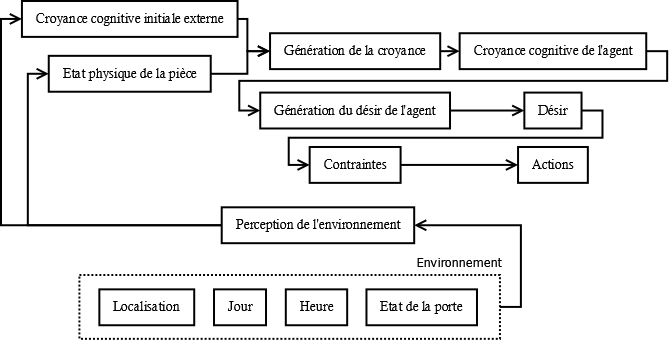
\includegraphics[scale=0.4]{Images/diagrammes_SMA/BRAHMS}
\caption{Diagramme représentant les éléments de la simulation sous BRHAMS pour la gestion de l'ouverture des portes}
\label{fig:Diagramme_BRAHMS}
\end{figure}

\subsection{Repast}

Repast (\textit{REcursive Porous Agent Simulation Toolkit}) est une plateforme de modélisation et simulation avancée, gratuite et libre à base d'agents initialement développée par l'\textit{University of Chicago}. Il existe deux éditions: \textit{Repast Simphony} développée en Java, interactive et relativement facile à utiliser et \textit{Repast HPC (High-Performance Computing)} développée en C++, à destination d'experts et nécessitant une excellente puissance de calcul.

Alfakara et Croxford \cite{Alfakara-14} utilisent Repast Simphony pour modéliser le comportement des occupants en confort estival dans les logements. Le modèle permet aux agents virtuels de Repast d'agir sur l'ouverture des fenêtres et sur l'activation de l'air conditionnée. La modélisation des occupants se base sur la création d'agents avec des propriétés individuelles (âge, style de vie, tolérance à la température, ...), autonomes et pouvant interagir entre eux. Le développement de ce modèle sous Repast permet par la suite d'étudier l'impact du comportement des occupants sur les consommations de climatisation. En effet, le SMA est couplé dynamiquement à un logiciel de simulation thermique, EDSL, qui traite le bâtiment et son environnement. Un objectif de cette étude est alors de comparer comment la manière de ce comporter vis à vis de la gestion des surchauffes modifie les consommations énergétiques. L'arbre décisionnel en Figure \ref{fig:Diagramme_Repast} montre le fonctionnement de général utilisé pour gérer les ouvertures de fenêtres et les actions sur la climatisation. Le processus décisionnel se présente alors comme un algorithme linéaire assez simple dans cet exemple, mais il peut être complexifié sans contrainte majeure. En amont de ce processus il est nécessaire de générer les agents et leurs propriétés intrinsèques.

\begin{figure}[H]
\centering
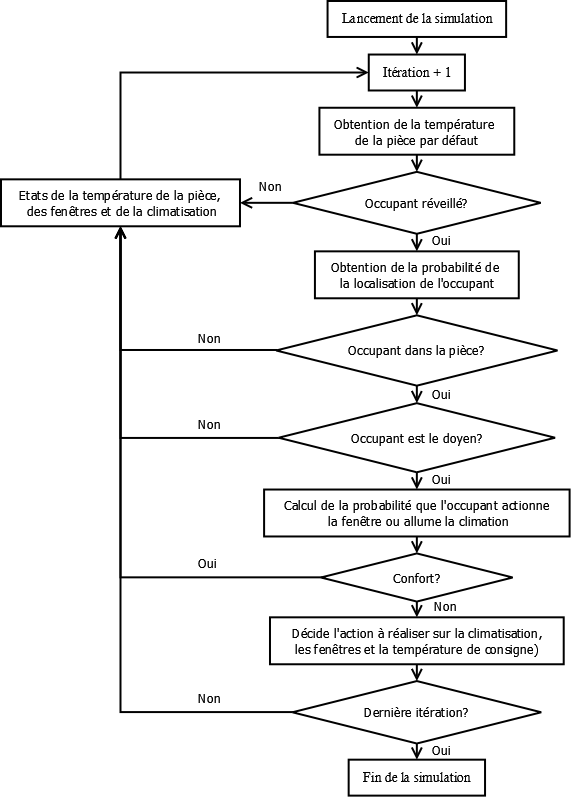
\includegraphics[scale=0.4]{Images/diagrammes_SMA/Repast}
\caption{Digramme décisionnel représentant les éléments de la simulation sous Repast pour la modélisation du confort estival}
\label{fig:Diagramme_Repast}
\end{figure}

\subsection{NetLogo}

NetLogo est une plateforme open-source SMA de modélisation de phénomènes collectifs. La plateforme est bien adaptée à la modélisation de systèmes complexes composés de centaines d'agents agissants en parallèle. La plateforme offre la possibilité de créer ses propres modèles constitués de trois types d'agents: les "\textit{turtles}" qui se déplacent dans leur environnement, les "\textit{patchs}" qui sont une portion statique de l'espace et les "\textit{observers}" qui organisent et donnent des instructions aux autres agents. NetLogo permet des modélisations des sciences sociales et naturelles de manière relativement simple.

Andrews et al. \cite{Andrews-11} ont utilisé NetLogo pour tester comment les bâtiments réagissent en fonction du comportements des occupants. Le comportement a été illustré sur l'application du confort des agents à la lumière et à son intensité. La modélisation du comportement des usagers sur la plateforme NetLogo doit pouvoir à terme être intégrée à une maquette numérique de type BIM. En effet, les limites du BIM peuvent être repoussées assez loin et une intégration des activités des occupants est à prévoir. Dans ces travaux, le lien est réalisé entre l'approche bien connue du BDI (\textit{Belief - Desire - Intension}) qui considère les croyances, les désires et les intentions des occupants et l'approche TPB (\textit{Theory of Planned Behaviour}) qui se base sur un modèle normalisé du comportement humain. L'objectif de ce couplage est alors de rendre la modélisation du comportement des occupants encore plus rationnelle que ce qui a l'habitude de se faire. La Figure \ref{fig:Diagramme_NetLogo} présente le processus décisionnel général correspondant qui mène à un comportement ou une action en utilisant la plateforme NetLogo. La modélisation dite de type \textit{BDI} est mise en évidence dans la première partie de l'algorithme puis la \textit{TPB} dans la deuxième, cela afin d'en définir l'état environnemental suivant.

\begin{figure}[H]
\centering
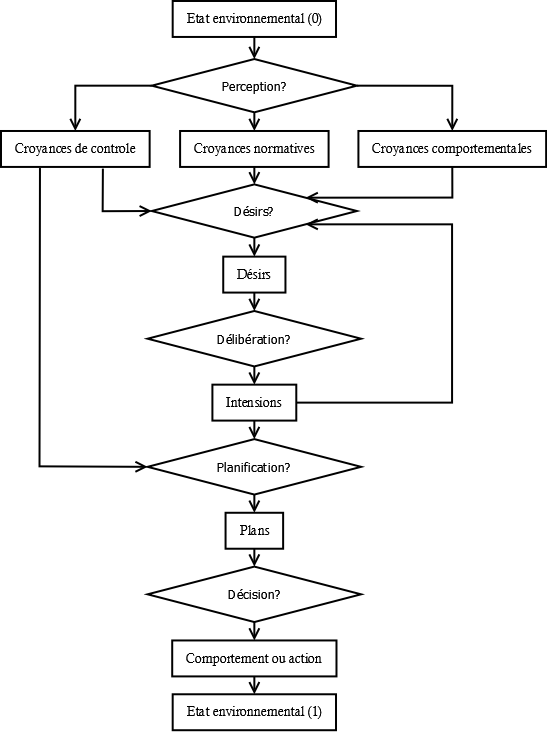
\includegraphics[scale=0.4]{Images/diagrammes_SMA/NetLogo}
\caption{Diagramme décisionnel représentant les éléments de la simulation sous NetLogo avec la combinaison \textit{BDI} et \textit{TPB}}
\label{fig:Diagramme_NetLogo}
\end{figure}

\subsection{OASys}

Cette sous-section est présentée différemment des autres puisque la plateforme OASys (\textit{Occupants’ Actions System}) fait partie de la deuxième catégorie de plateforme présentée dans ce chapitre. En effet, le développement par l'Université de Toulouse d'OASys a été codé sous JAVA pour ensuite être couplé à TRNSYS via C++. La modélisation du comportement des occupants n'utilise alors pas de plateforme pré-existante comme les travaux d'Andrews et al. \cite{Andrews-11}, d'Alfakara et Croxford \cite{Alfakara-14} ou encore de Tijani \cite{Tijani-14}.

Le cœur de la modélisation de Bonte \cite{Bonte-14} est basé sur le confort des occupants via un algorithme d'intelligence artificielle. Le modèle permet alors de prendre en compte les préférences interindividuelles et la simulation des actions des occupants en fonction de leurs sensations thermiques ou visuelles. Bonte couple par la suite la plateforme OASys avec le logiciel de Simulation Thermique Dynamique TRNSYS pour étudier l'influence du comportement des occupants sur la performance énergétique des bâtiments. La Figure \ref{fig:Diagramme_OASys} représente les éléments modélisés de la simulation sous OASys. Cela permet de bien visualiser que la modélisation de la part humaine est réalisée en deux étapes. Premièrement l'état physiologique est évalué par des modèles de confort thermiques et visuelles, et ensuite une réaction comportementale associée à une action est transmise à l'outil de STD pour en modifier l'environnement intérieur.

\begin{figure}[H]
\centering
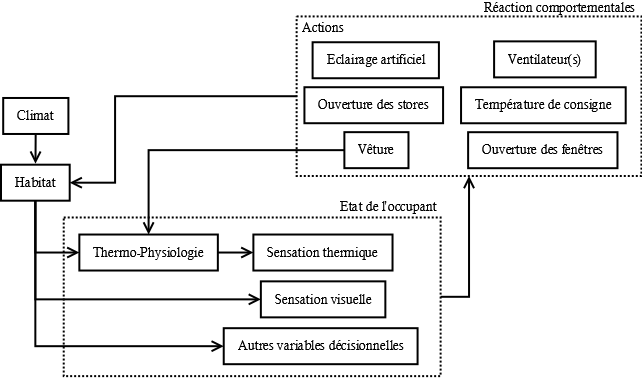
\includegraphics[scale=0.4]{Images/diagrammes_SMA/OASys}
\caption{Diagramme représentant les éléments de la simulation sous OASys avec la mise en avant de l'importance du confort}
\label{fig:Diagramme_OASys}
\end{figure}

\subsection{MASS}
\label{FlowchartInternMASS}

Comme OASys, MASS (\textit{Multi-Agents Stochastic Simulation}) est une plateforme développée sans l'utilisation de plateforme SMA générale, mais développée sous C++ sur-mesure à la modélisation des individus dans les bâtiments. 

Le concept de plateforme multi-agent est originellement issu des travaux de Robinson et al. \cite{Robinson-11} et a pour objectif de réduire le \textit{performance gap} en améliorant la modélisation des occupants. Cette idée, développée par l'Ecole Polytechnique Fédérale de Lausanne puis par l'Université de Nottingham, prend en compte les actions des occupants et leur nature imprévisible afin d'être couplée à des outils simulation thermique dynamique. Chapman et al. \cite{Chapman-14} proposent par la suite une version restructurée, baptisée MASS, qui fonctionne en co-simulation avec EnergyPlus ainsi qu'avec une de ces interface utilisateur DesignBuilder. Le développement de MASS, a été réalisé par l'utilisation de sous-modèles issus notamment des travaux de Page et al \cite{Page-08}, Haldi et Robinson \cite{Haldi-09} \cite{Haldi-10}. La Figure \ref{fig:Diagramme_MASS} présente le diagramme décisionnel général du modèle MASS, celui-ci nous permet de mieux visualiser les différents composants de la plateforme. L'algorithme de MASS se compose de deux parties distinctes: la première permet le pré-processus de la simulation afin de fixer les paramètres fixes et la seconde permet l'échange de données, présence et actions, avec l'outil de simulation du bâtiment.

\begin{figure}[H]
\centering
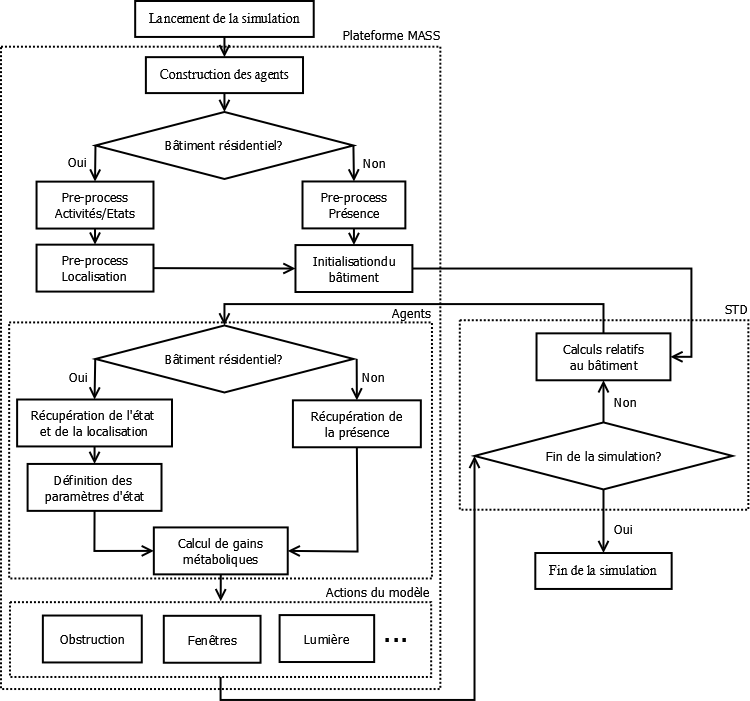
\includegraphics[scale=0.4]{Images/diagrammes_SMA/MASS}
\caption{Diagramme décisionnel représentant les éléments de la simulation sous MASS et la liaison avec EnergyPlus}
\label{fig:Diagramme_MASS}
\end{figure}

\subsection{Composant W de TRNSYS}

Nous venons donc de présenter cinq plateformes multi-agents, dans l'objectif de trouver le moyen le plus approprié d'améliorer la prise en compte des occupants dans les STD. Néanmoins notre attention a également longtemps été portée sur l'approche qui consiste à personnaliser le code (cf section \ref{Le simulateur personnalise le code}). La comparaison de cette approche, basé sur l'exemple du composant W de TRNSYS, avec la co-simulation nous a permis d'identifier certaine limites et de s'assurer que le couplage n'ajoutait pas de la complexité inutilement.

Les avantages de l'utilisation d'un composant comme le langage W proposé par TRNSYS sont multiples. Premièrement, il permet de travailler dans un environnement de programmation simple, sans compilateur et sur un logiciel convivial. Deuxièmement, l'utilisation  qui peut être réalisée est techniquement accessible pour les bureaux d'études qui ne sont généralement pas prêt à travailler sans interface utilisateur. Aussi, l'investissement en temps étant très largement inférieur à celui qui consiste à développer une plateforme externe, permet à priori de réaliser davantage d'études. Enfin, l'investissement économique est très raisonnable, en comparaison au prix du logiciel et de la bibliothèque TESS \footnote{TESS pour \textit{Thermal Energy System Specialists} est une bibliothèque très utile pour réaliser des études complexes et étendre les fonctionnalités d TRNSYS}, puisque le langage W ne coûte que 195 \euro{} \footnote{http://boutique.cstb.fr/Product/langage-w}. 

Néanmoins, les limitations de l'utilisation de cette bibliothèque TRNSYS (Version 17) existent. En effet, malgré les mérites vendus sur la modularité et l'extensibilité de TRNSYS par le CSTB (le revendeur du logiciel), les possibilités de développements ne sont pas illimitées. Sans l'utilisation d'autres logiciels ou bibliothèques, il n'est par exemple pas possible d'obtenir le niveau d'éclairement d'une zone. Cet élément manquant, présent sur EnergyPlus (Version 8.2), est très pénalisant pour les modèles de gestion de stores et d'éclairage artificiel qui l'utilisent dans la plus part des cas. La simple génération de nombres aléatoires sur une distribution rectangle ou normale n'est pas possible au sein du langage W. Pour obtenir ces nombres, il est nécessaire d'utiliser un générateur issu de la bibliothèque TESS, puis de les renvoyer vers les modèles écrit dans W. Le caractère extensible de TRNSYS est donc bien amélioré avec le langage W, mais n'est à notre sens pas optimisé comme peut l'être un langage de bas niveau.

L'ensemble des outils permettant de modéliser les comportements à base de SMA sont synthétisés dans le Tableau \ref{tab:syntheseSMA}. Ce Tableau permet notamment de révéler la diversité des outils utilisés et la maturation des projets pour une application industrielle.

\begin{table}
\begin{center}
\begin{tabular}{{|p{3cm}||p{2.5cm}|p{2.5cm}|p{3.5cm}|p{3.5cm}|}}
\hline Plateforme - [Référence] & Reprise d'une plateforme générale & Outils STD & Potentiel de finesse de la modélisation & Fonctionnalité en BE \\
\hline
\hline BRAHMS - \newline Tijani et al. \cite{Tijani-14} & Oui & Non couplé (?) & Très fin - basé sur les sciences cognitives & Quasi impossible: demande un énorme travail \\
\hline Repast - \newline Alfakara et al. \cite{Alfakara-14} & Oui & EDSL 2012 & Moyen - basé sur le bon sens du modélisateur & Non - Application spécifique au confort estival \\
\hline NetLogo - \newline Andrews et al. \cite{Andrews-11} & Oui & MATLAB & Fin - basé sur les théories \textit{BDI} et \textit{TPB} & Possible - Modèle comportemental à simplifier \\
\hline OASys - \newline Bonte et al. \cite{Bonte-14} & Non & TRNSYS & Fin  - basé sur le confort thermique et visuel & Modèle comportemental à simplifier \\
\hline MASS - \newline Chapman et al. \cite{Chapman-14} & Non & EnergyPlus & Moyen - basé sur des comportements réactifs & Assez difficilement à l'heure actuelle \\
\hline Composant W & Non & TRNSYS & Grossier - L'impossibilité d'insérer des bibliothèques bride le développement & Totale \\
\hline
\end{tabular}
\caption{Synthèse des modèles à base d'agents servant à créer un lien avec un outil STD}
\label{tab:syntheseSMA}
\end{center}
\end{table}

\section{Synthèse}

L'approche consistant à modéliser le comportement des occupants à partir de modèles déterministes a été repoussée pour des raisons de représentativité des comportements réels. Les modèles stochastiques correspondent bien à nos attentes, car ils permettent de reproduire le caractère aléatoire des décisions humaines. Néanmoins, les systèmes multi-agents, issus de l'intelligence artificielle, ont également été appréciés. Ils permettent d'une part d'intégrer des modèles stochastiques et d'autre part de faire interagir les occupants et de considérer leur confort. Après avoir présenté quatre moyens d'intégrer des modèles de comportement dans des logiciels de simulation thermique dynamique, nous avons comparé des études qui utilisent des plateformes similaires à ce que nous souhaitons. Une première option consistait donc à utiliser une plateforme multi-agents générale afin de posséder une bonne liberté de développement, cela étant lourd en terme d'investissement et éloigné de l'objectif d'amélioration des outils de STD. La seconde option est la plus rapide et simple à mettre en place, elle consiste à intégrer directement de nouveaux modèles dans les outils existants mais en négligeant totalement les interactions humaines, le confort et étant sans modularité. La dernière option consistait à développer et co-simuler un environnement unique composé de l'ensemble des modèles comportementaux nécessaires avec un outil de simulation. En outre pour des raisons de potentiel de l'outil nous avons opté pour la troisième option.

A l'issu de ce travail bibliographique et de définition des moyens, nous avons contacté l'Université de Nottingham pour proposer une collaboration. En effet, cette Université a débuté ce type de recherche dans les années 2000 et possède une expertise très estimable. La demande a été acceptée et a débouchée sur une visite et une présentation de leur outil MASS (\textit{Multi-Agents Stochastic System}). Outil que nous avons "adopté" par la suite et qui est utilisé comme base de travail dans la suite de la thèse.
